
\begin{frame}[fragile]
  \begin{block}{Example Syntax}\pause
  \begin{lstlisting}
x <- x[-1, 2:5]
x <- log(abs(x) + 1)
xtx <- t(x) %*% x
ans <- svd(solve(xtx))
  \end{lstlisting}
  \begin{center}
  \pause Look familiar?\\[.4cm] \pause
  \emph{The above runs on 1 core with R or 10,000 cores with pbdR}
  \end{center}
  \end{block}
\end{frame}


\begin{frame}
  \begin{block}{Least Squares Benchmark}\pause
  \begin{center}
  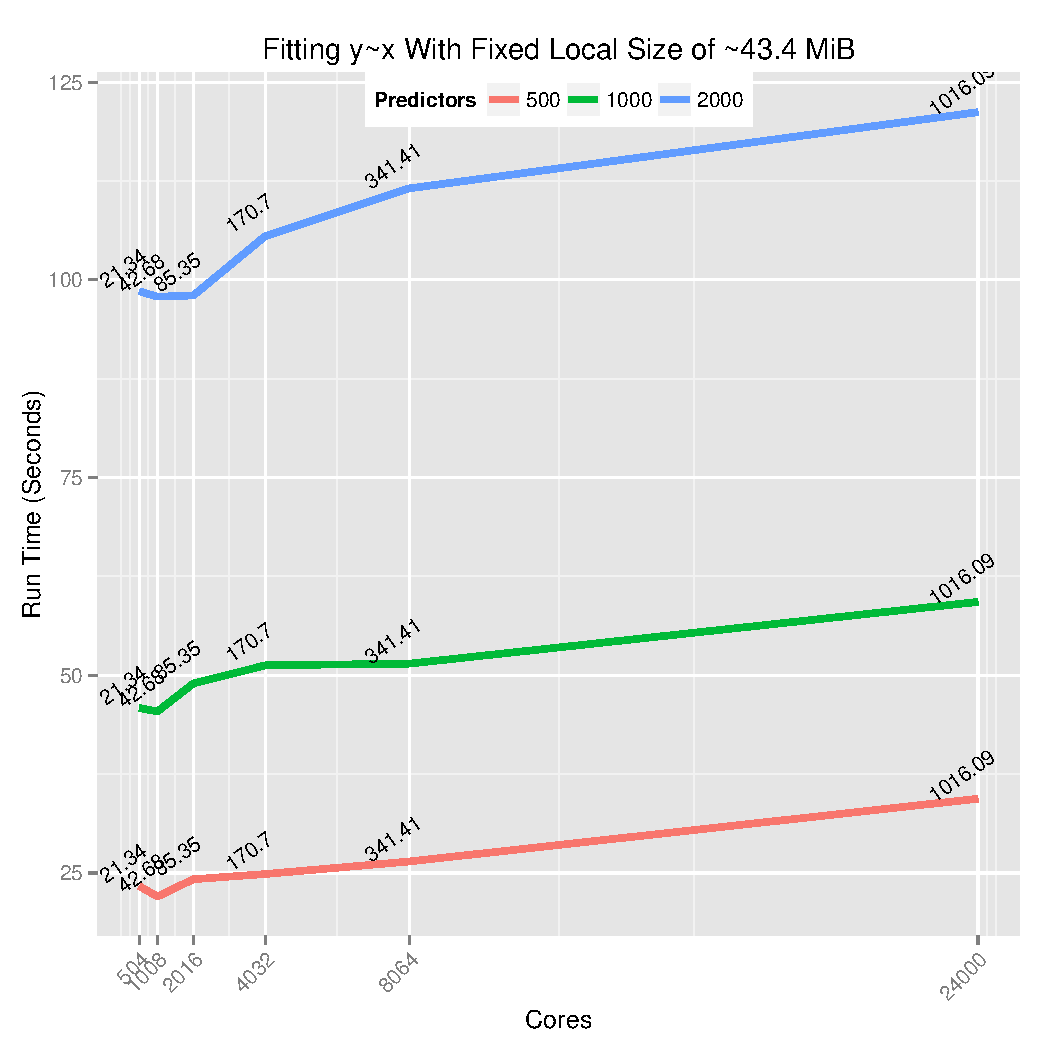
\includegraphics[height=.89\textheight]{../common/pics/benchmarks/lmfit2}
  \end{center}
  \end{block}
\end{frame}

